%Latex document for ESSDERC 2021 Paper 

\documentclass[11pt,a4paper,twocolumn]{article}
\usepackage[utf8]{inputenc}
\usepackage{authblk}
\usepackage{amsmath}
\usepackage{amsfonts}
\usepackage{amssymb}
\usepackage{makeidx}
\usepackage{graphicx}
\usepackage{fourier}
\usepackage[ruled,vlined]{algorithm2e}
\usepackage{empheq}

\usepackage[left=2cm,right=2cm,top=2cm,bottom=2cm]{geometry}

% Title
\title{3D Simulation of PDE and Jitter in SPAD Devices.}

% AUthors and affiliation
\author[1]{Rémi Helleboid}
\author[1]{Denis Rideau}
\author[1]{Jeremy Grebot}
\author[2]{Norbert Moussy}
\author[2]{Olivier Saxod}
\affil[1]{ST Microelectronics, Crolles, France}
\affil[2]{CEA LETI, Grenoble, France}

\date{}                     %% To hide the date
\setcounter{Maxaffil}{0}
\renewcommand\Affilfont{\itshape\small}
% Keywords command
\providecommand{\keywords}[1]
{
  \small	
  \textbf{\textit{Keywords---}} #1
}


\begin{document}


% Title
\maketitle

% Abstract
\begin{abstract}
In this paper we present a full 3D simulation methodology to extract Photon Detection Probability (PDP) and Jitter of Single-Photon Avalanche Diode (SPAD) Devices. The simulation results are compared with measurements on devices and show good agreement with the experiments.\\
\end{abstract}

% Keywords
\keywords{single-photon avalanche diode (SPAD), photon detection probability (PDP), jitter, avalanche breakdown probability, breakdown voltage}

% Introduction
\section{Introduction}
Single-photon avalanche diodes (SPADs) are key opto-electronics devices.


\section{Device structure and TCAD simulation}
\begin{figure}[hbtp]
\caption{SPAD simulation workflow}
\centering
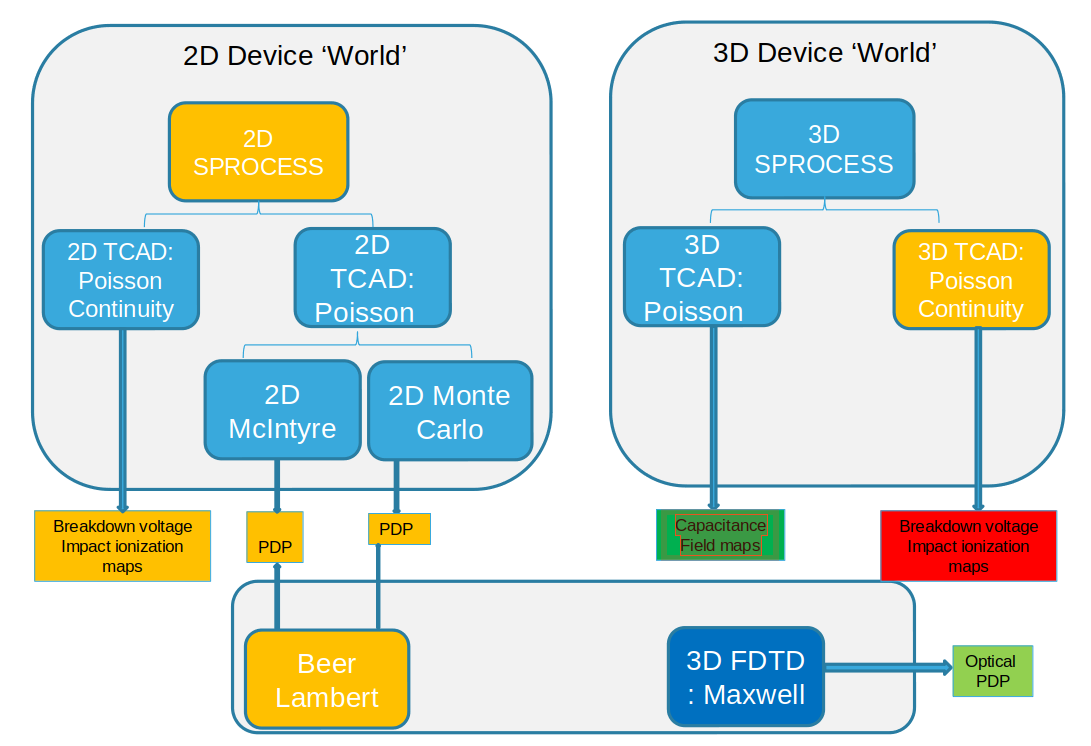
\includegraphics[scale=0.21]{../pictures/TCADWorkflow.png}
\end{figure}


\section{Avalanche breakdown probability}
The avalanche breakdown probability is computed by the means of the well known McIntyre model \cite{oldham_triggering_1972}. We briefly recall the model derivation : 
Let $P_e(x)$ be the probability that an electron starting at x in the depletion layer triggers an avalanche and $P_h(x)$ the same probability for an hole starting at x.
Straightforwardly, the probability that neither an hole nor an electron starting at x trigger an avalanche is given by $(1-P_e(x))(1-P_h(x))$.
Thus, the probability that either the hole or the electron trigger an avalanche, noted $P_{pair}$ is :
\begin{align*}
P_{pair}(x) &= 1 - \left( 1-P_e(x)\right)\left(1-P_h(x)\right)  \\
			&= P_e + P_h - P_e P_h
\end{align*}

Now, the probability that an electron starting at $x+dx$ triggers an avalanche is :
The probability that the electron reaches the position $x$ and triggers an avalanche in $x$ plus the probability that it triggers an avalanche between $x$ and $x+dx$ less the probability of the intersection of the two previous events. It writes : 
\begin{align*}
P_e(x+dx) &= P_e(x) + \alpha_e(x) dx P_{pair}(x)  - P_e(x)  \alpha_e dx P_{pair}(x) \\
		  &= P_e(x) + \alpha_e(x) dx (P_e(x) + P_h(x) - P_e(x) P_h(x)) \\& \qquad - P_e(x) \alpha_e(x) dx (P_e(x) + P_h(x) - P_e(x) P_h(x)) \\
		  &=  P_e(x) + dx \, \alpha_e(x) (P_e(x) + P_h(x) - P_e(x) P_h(x)) (1 - P_e(x))
\end{align*}
Where $\alpha_e$ is the electron linear ionization rate : the probability by length that an electron create an impact ionization event.  \\
One can rearrange the terms to obtain : 
\[ \frac{P_e(x+dx)-P_e(x)}{dx} = \alpha_e(x) (P_e(x) + P_h(x) - P_e(x) P_h(x)) (1 - P_e(x)) \]
Which leads to the first ordinary differential equation : 
\[ \frac{dP_e}{dx} = (1-P_e)\alpha_e(P_e + P_h - P_e  P_h) \]

The same reasoning applies to the probability that an hole starting at $x-dx$ triggers an avalanche.
Which leads to the second ordinary differential equation : 
\[ \frac{dP_h}{dx} = -(1-P_h)\alpha_h(P_e + P_h - P_e  P_h) \]

Therefore we can draw up the McIntyre system : 

\begin{empheq}[left=\empheqlbrace]{align}
&\frac{dP_e}{dx} = (1-P_e)\alpha_e(P_e + P_h - P_e  P_h) \\
&\frac{dP_h}{dx} = -(1-P_h)\alpha_h(P_e + P_h - P_e  P_h) 
\end{empheq}
for $ 0 \leq x \leq W$. \\
Adding the couple of boundary value conditions
 : 
\begin{empheq}[left=\empheqlbrace]{align}
& P_e(x=0) = 0 \\
& P_h(x=W) = 0 
\end{empheq}
we have a full 1D coupled and non-linear boundary value problem.
Since we have to extract this value at a large number of points, we use a self-made solver, embedded in a C++ program. This solver uses finite difference method coupled with a Newton's method to care of the non-linearity of the problem. The algorithm is different from those implemented in MatLab routine $\textrm{(bvp4c)}$ or SciPy function $\textrm{(solve\_bvp)}$  but the comparison with these tools show no difference.


\begin{figure}[h]
\caption{Field line of electric field inside the device}
\centering
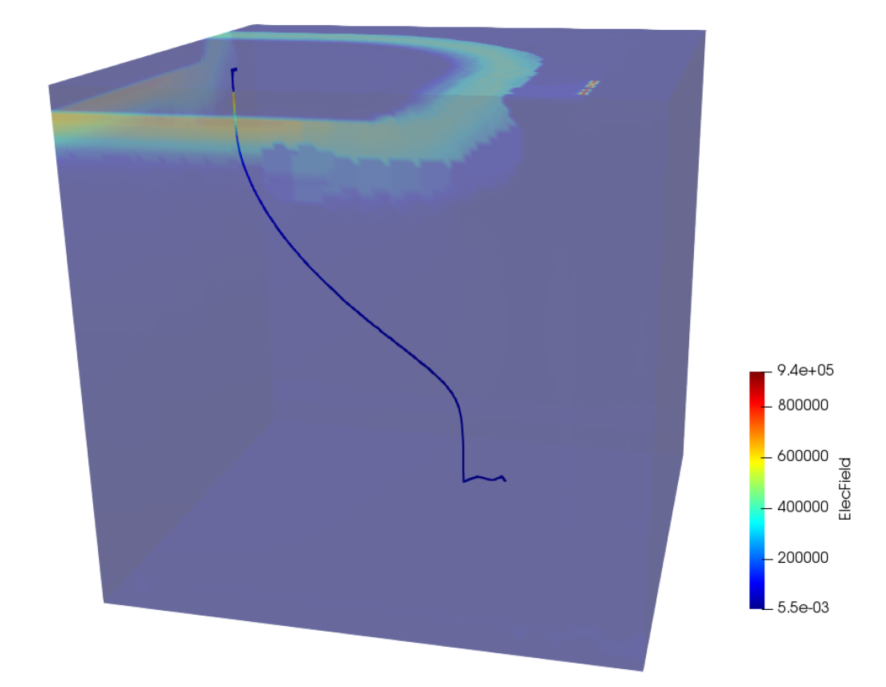
\includegraphics[scale=0.4]{../pictures/SL1.png}
\end{figure}


\IncMargin{1em}
\begin{algorithm}[h]
	\SetKwData{Left}{left}
	\SetKwData{This}{this}
	\SetKwData{Up}{up}
	\SetKwFunction{Union}{Union}
	\SetKwFunction{FindCompress}{FindCompress}
	\SetKwInOut{Input}{input}\SetKwInOut{Output}{output}
	\Input{The Boundary value Problem}
	\Input{The Mesh $\mathcal{M}$}
	\Input{An initial guess of $Y_{\mathcal{M}}$}
	\Input{A maximal tolerance TOL}
	\Input{A maximal number of iterations}
	\Output{The Solution  $Y_{\mathcal{M}}$}
	\Output{The final residual error }
	\BlankLine
	$\text{RES} \leftarrow  1000$ \;
	$NbIterations \leftarrow 0$\;
	Initialize $w_{\mathcal{M}}$ as a vector of size 2N\;
	\BlankLine
	\While{$RES > TOL$ and NbIterations < MaxNbIterations}{
		\For{i=1 to 2N}{
			Construct $S_i$\;
			Construct $R_i$\;
		 	Construct $q_i =-\textbf{N}_{\mathcal{M}}y_i$\;	}
		Construct $A$\;
		Construct $\beta$\;
		\BlankLine
		Solve $A  w_{\mathcal{M}} = \hat{\beta}$\;
		\BlankLine
		{\For{i=1 to 2N}
			{$y_i \leftarrow y_i + \left( w_{\mathcal{M}}\right)_i $ }}
		\BlankLine
		$RES \leftarrow ||w_{\mathcal{M}}||$\;
		$NbIterations \leftarrow NbIterations + 1$\;
	}
	\If{$RES \leq TOL$}{
		//The method has converged \;
		\Return	Y\;
	}
	\Else{
		//The method has converged \;
		\Return Error : No Convergence
	}
	
	
\caption{Newton's Method Solver for BVP}\label{algo_newton}
\end{algorithm}
\DecMargin{1em}

\section{Jitter modeling}

\section{Results and comparisons with experiments}

\section{Discussion}

\newpage
\newpage
\nocite{*}
\bibliographystyle{apalike}
\bibliography{../biblio/essderc2k21}


















\end{document}